\chapter{Ficha técnica comparativa}

A continuación se recoge la ficha técnica comparada de las tres CVE seleccionadas. Todos los datos se han extraído directamente de los registros oficiales de la NVD (\texttt{nvd.nist.gov/vuln/detail/...}) y, cuando ha sido necesario, contrastados con los avisos del propio fabricante. En las figuras \ref{fig:cve1}, \ref{fig:cve2} y \ref{fig:cve3} se muestran las páginas de detalle de cada CVE en la NVD.

\begin{table}[H]
\centering
\renewcommand{\arraystretch}{1.35}
\footnotesize
\begin{tabularx}{\textwidth}{|>{\bfseries}p{3.6cm}|X|X|X|}
\hline
\rowcolor{lightblue}
\textbf{Campo} & \textbf{CVE 1} & \textbf{CVE 2} & \textbf{CVE 3} \\ \hline
Identificador CVE & CVE-2018-6350 & CVE-2025-53766 & CVE-2023-51582 \\ \hline
Plataforma / S.O. afectado & Android, iOS y Windows Phone (vía WhatsApp) & Microsoft Windows (componente nativo GDI+) & Linux (servicio Voltronic Power ViewPower / LinuxMonitorConsole) \\ \hline
Versiones afectadas & WhatsApp para Android $<$ 2.18.276; WhatsApp Business Android $<$ 2.18.99; WhatsApp para iOS $<$ 2.18.100.6; WhatsApp Business iOS $<$ 2.18.100.2; WhatsApp Windows Phone $<$ 2.18.224 & Múltiples ediciones de Windows 10/11 y Windows Server donde se distribuye GDI+ (consultar matriz de \textit{Security Update Guide} de Microsoft) & Voltronic Power ViewPower 1.04-22165 y anteriores (componente LinuxMonitorConsole) \\ \hline
CVSS Base Score & 9.8 (\textit{Critical}) & 9.8 (\textit{Critical}) & 9.8 (\textit{Critical}) \\ \hline
Vector CVSS completo & CVSS:3.0/AV:N/AC:L/PR:N\-/UI:N/S:U/C:H/I:H/A:H & CVSS:3.1/AV:N/AC:L/PR:N\-/UI:N/S:U/C:H/I:H/A:H & CVSS:3.0/AV:N/AC:L/PR:N\-/UI:N/S:U/C:H/I:H/A:H \\ \hline
Estado en NVD & \textit{Modified} (registro reanalizado el 09/03/2025) & \textit{Analyzed} & \textit{Modified} (última revisión el 07/09/2025) \\ \hline
¿CISA KEV? & No & No & No \\ \hline
¿PoC público? & No documentado públicamente (fix interno de Facebook) & No documentado de forma oficial; ya existen análisis técnicos del parche en blogs especializados & Sí: \textit{advisory} \texttt{ZDI-23-1887} de Zero Day Initiative \\ \hline
Fecha del primer parche oficial & Versiones de WhatsApp publicadas entre julio y agosto de 2018 & 12 de agosto de 2025 (\textit{Patch Tuesday}) & Versión 1.04-22169 de Voltronic Power ViewPower (mayo de 2024) \\ \hline
¿Era 0-day al publicarse? & No. La vulnerabilidad fue corregida por el fabricante antes de la publicación del CVE en 2019. & No. Se publicó dentro del ciclo coordinado de \textit{Patch Tuesday}, con el parche disponible el mismo día. & No. Reportada de forma coordinada a través del programa ZDI; el aviso público se liberó tras la disponibilidad del parche. \\ \hline
\end{tabularx}
\caption{Ficha técnica comparativa de las tres vulnerabilidades.}
\end{table}

\begin{figure}[H]
    \centering
    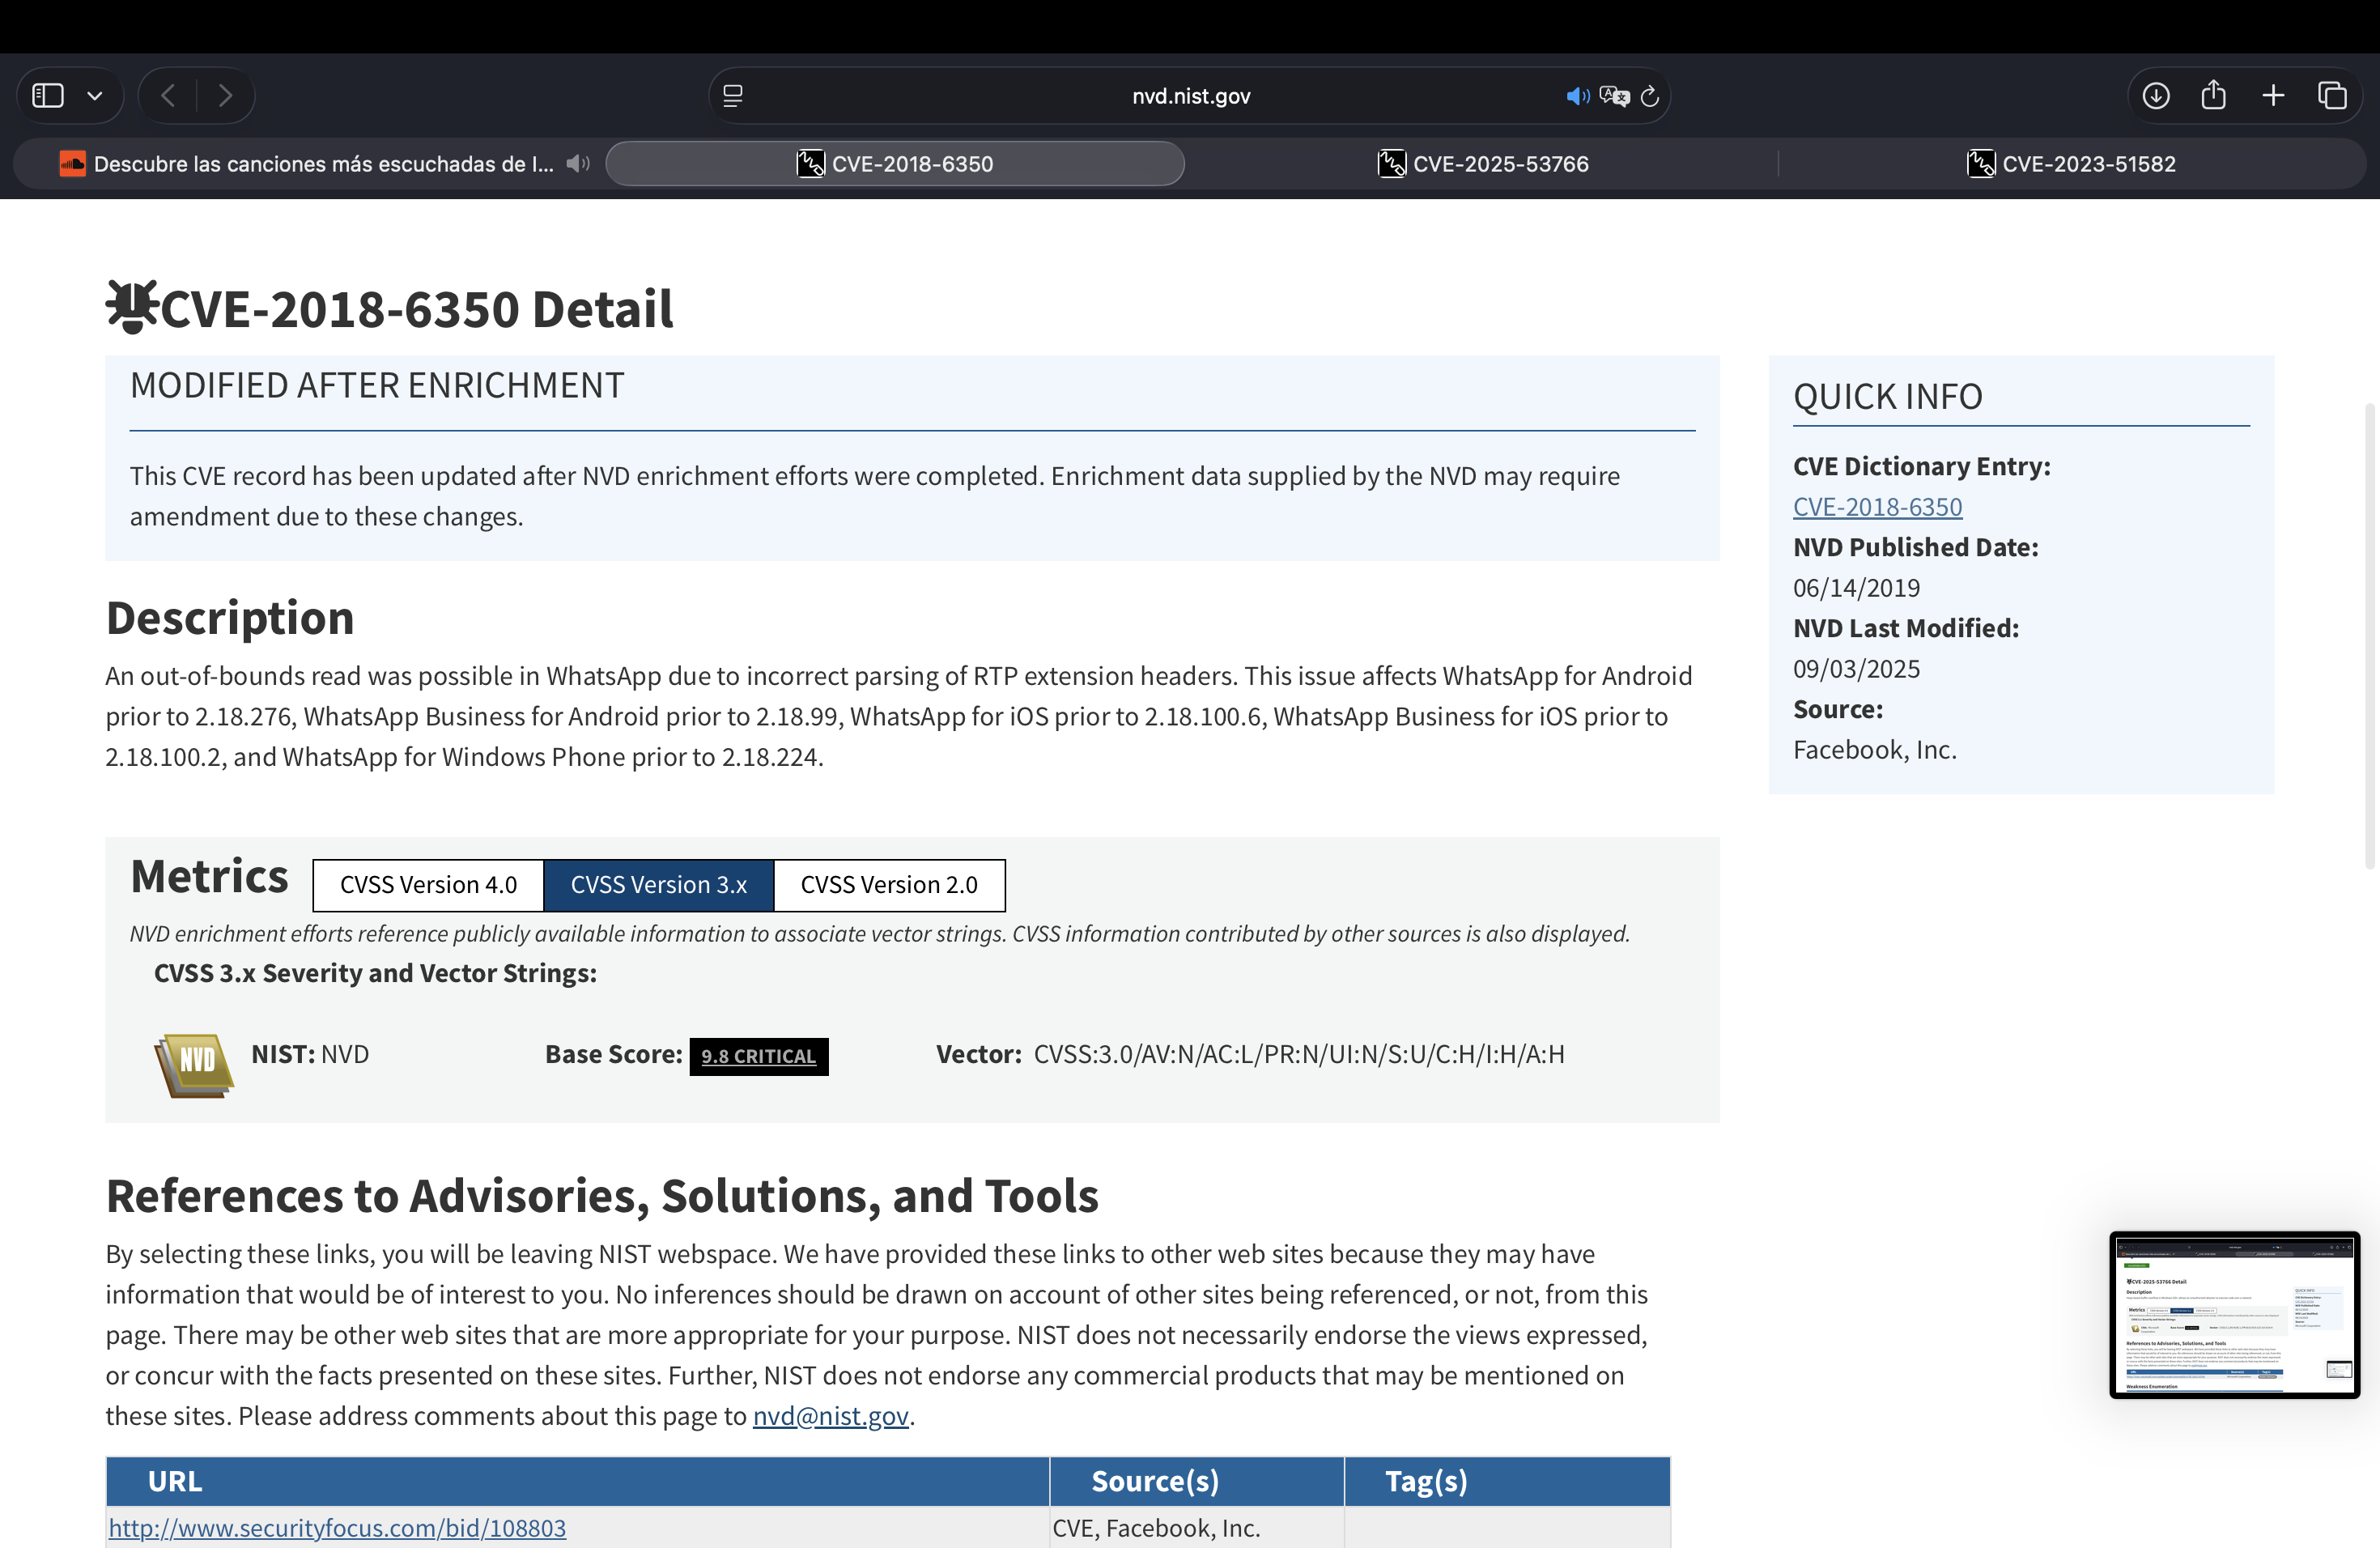
\includegraphics[width=0.95\textwidth]{Imagenes/05-CVE-1.png}
    \caption{Detalle de la CVE-2018-6350 en la NVD.}
    \label{fig:cve1}
\end{figure}

\begin{figure}[H]
    \centering
    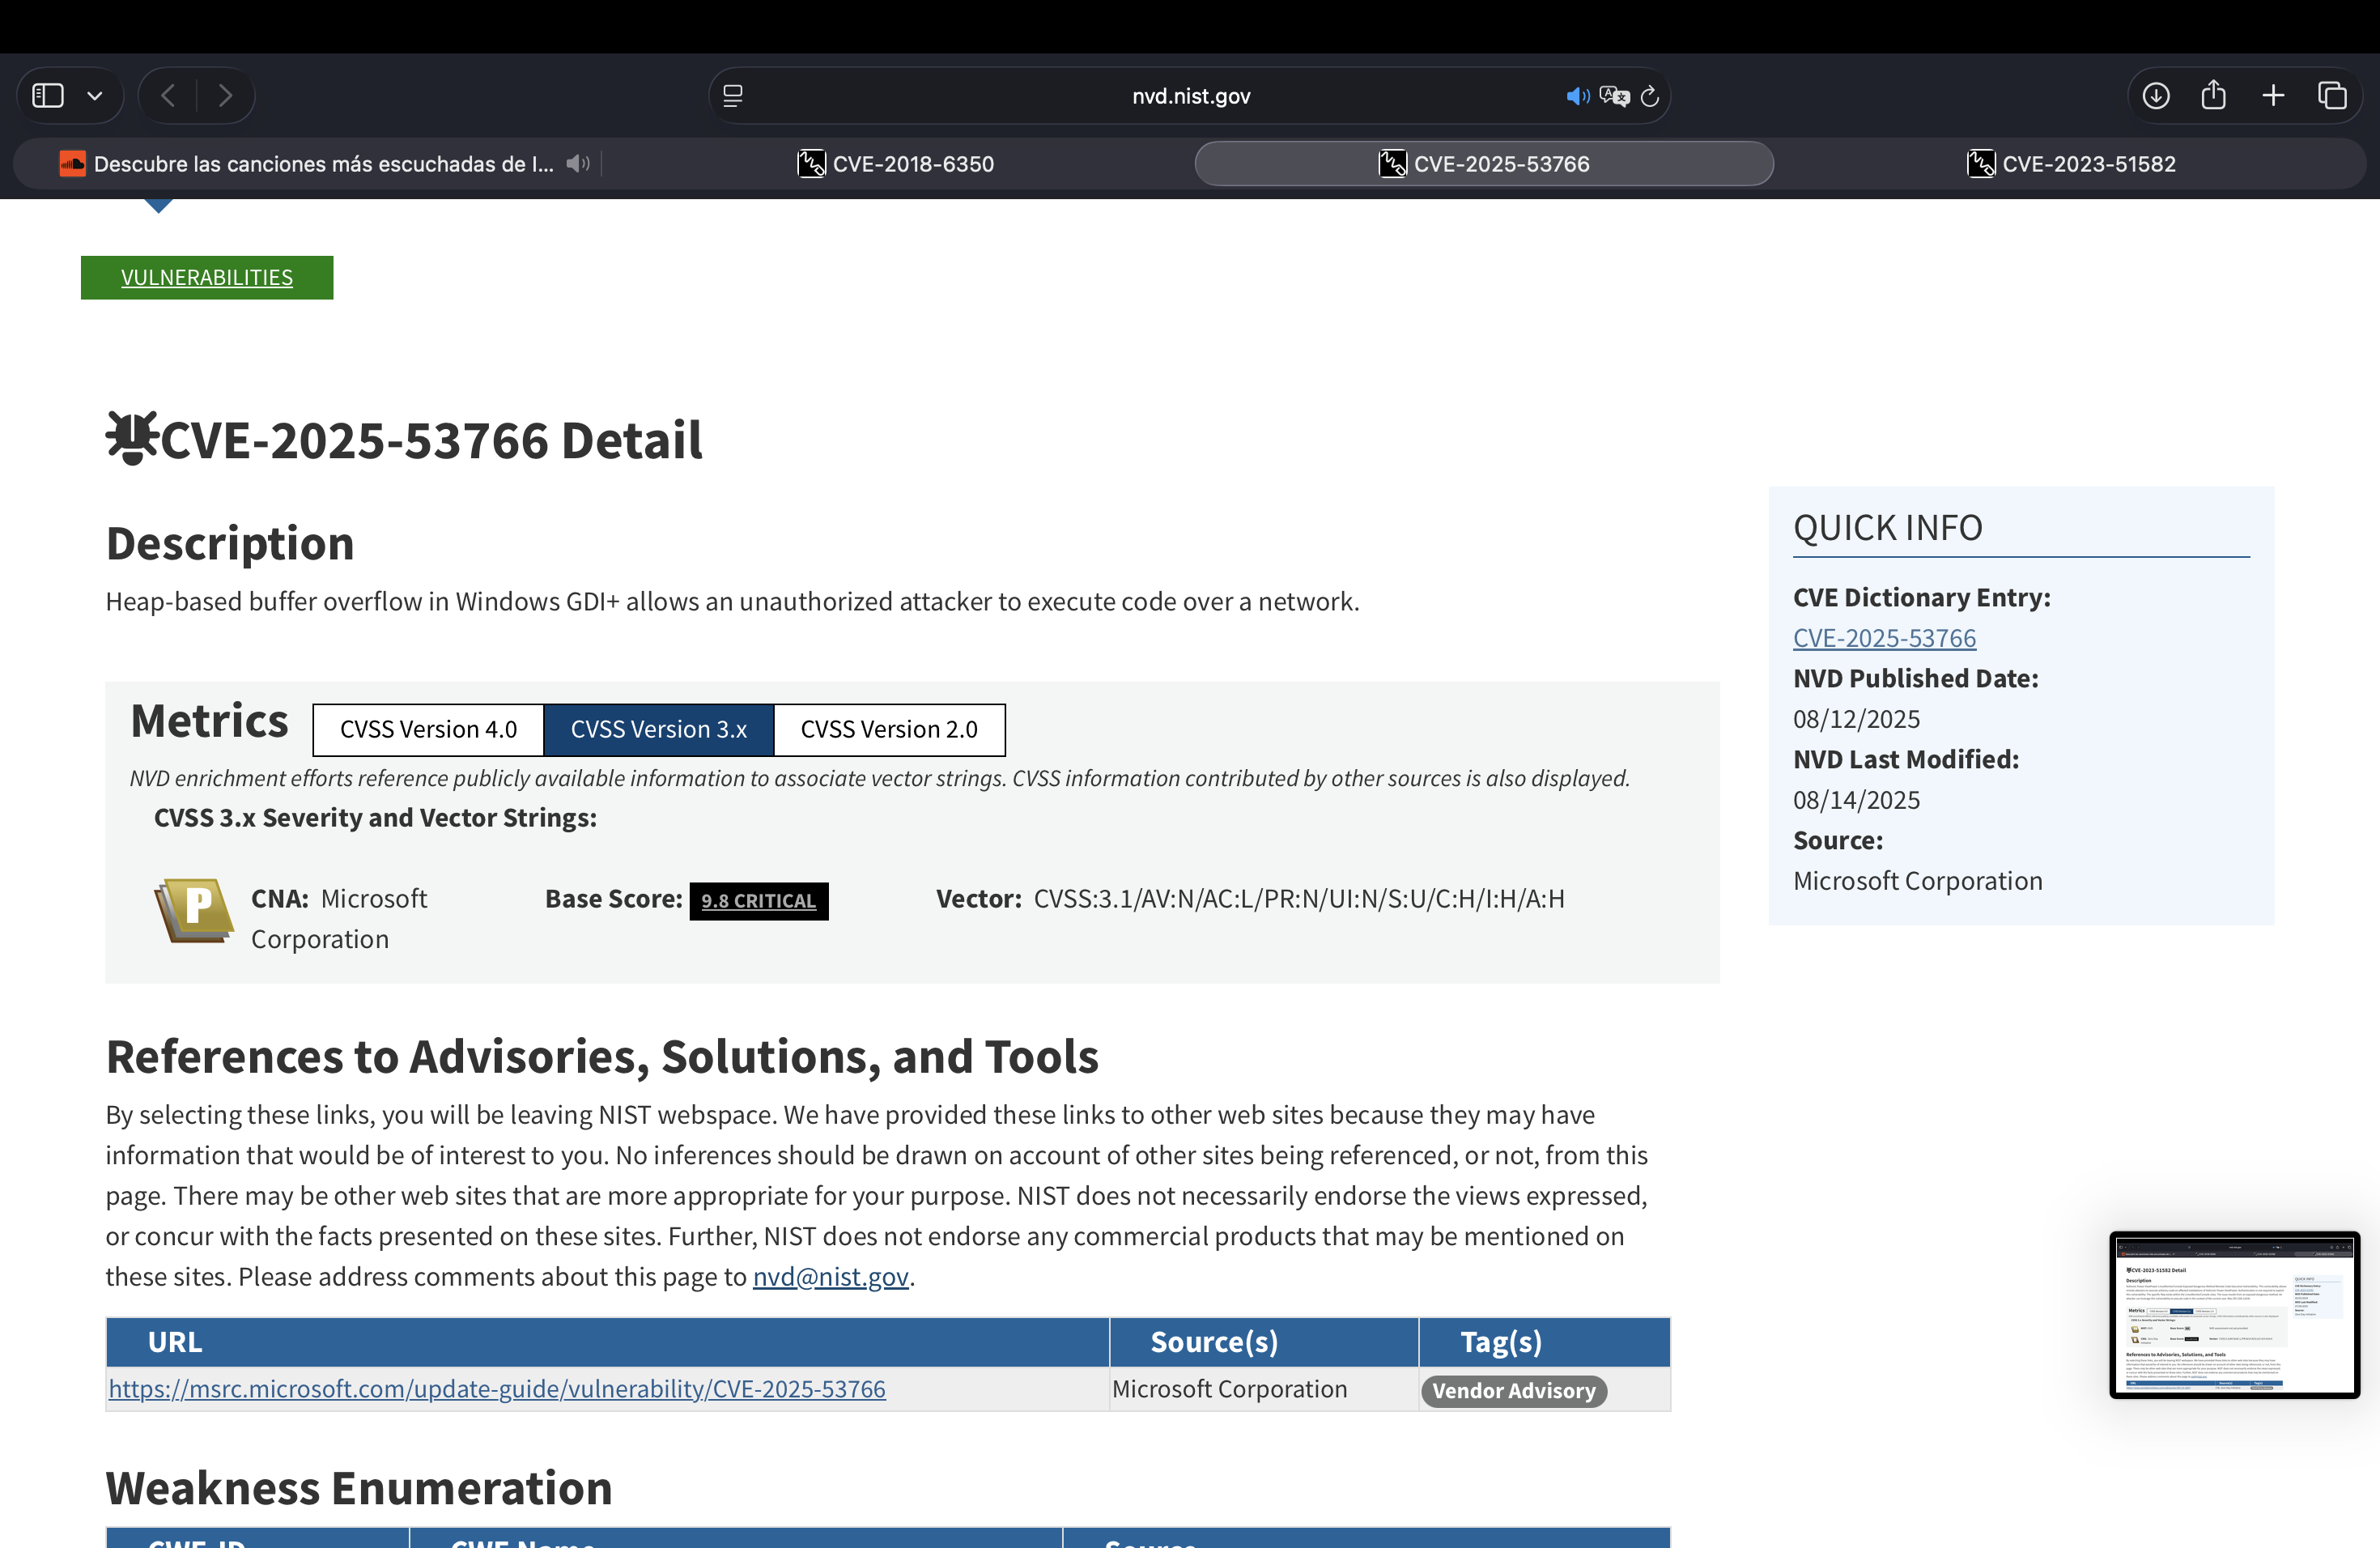
\includegraphics[width=0.95\textwidth]{Imagenes/06-CVE-2.png}
    \caption{Detalle de la CVE-2025-53766 en la NVD.}
    \label{fig:cve2}
\end{figure}

\begin{figure}[H]
    \centering
    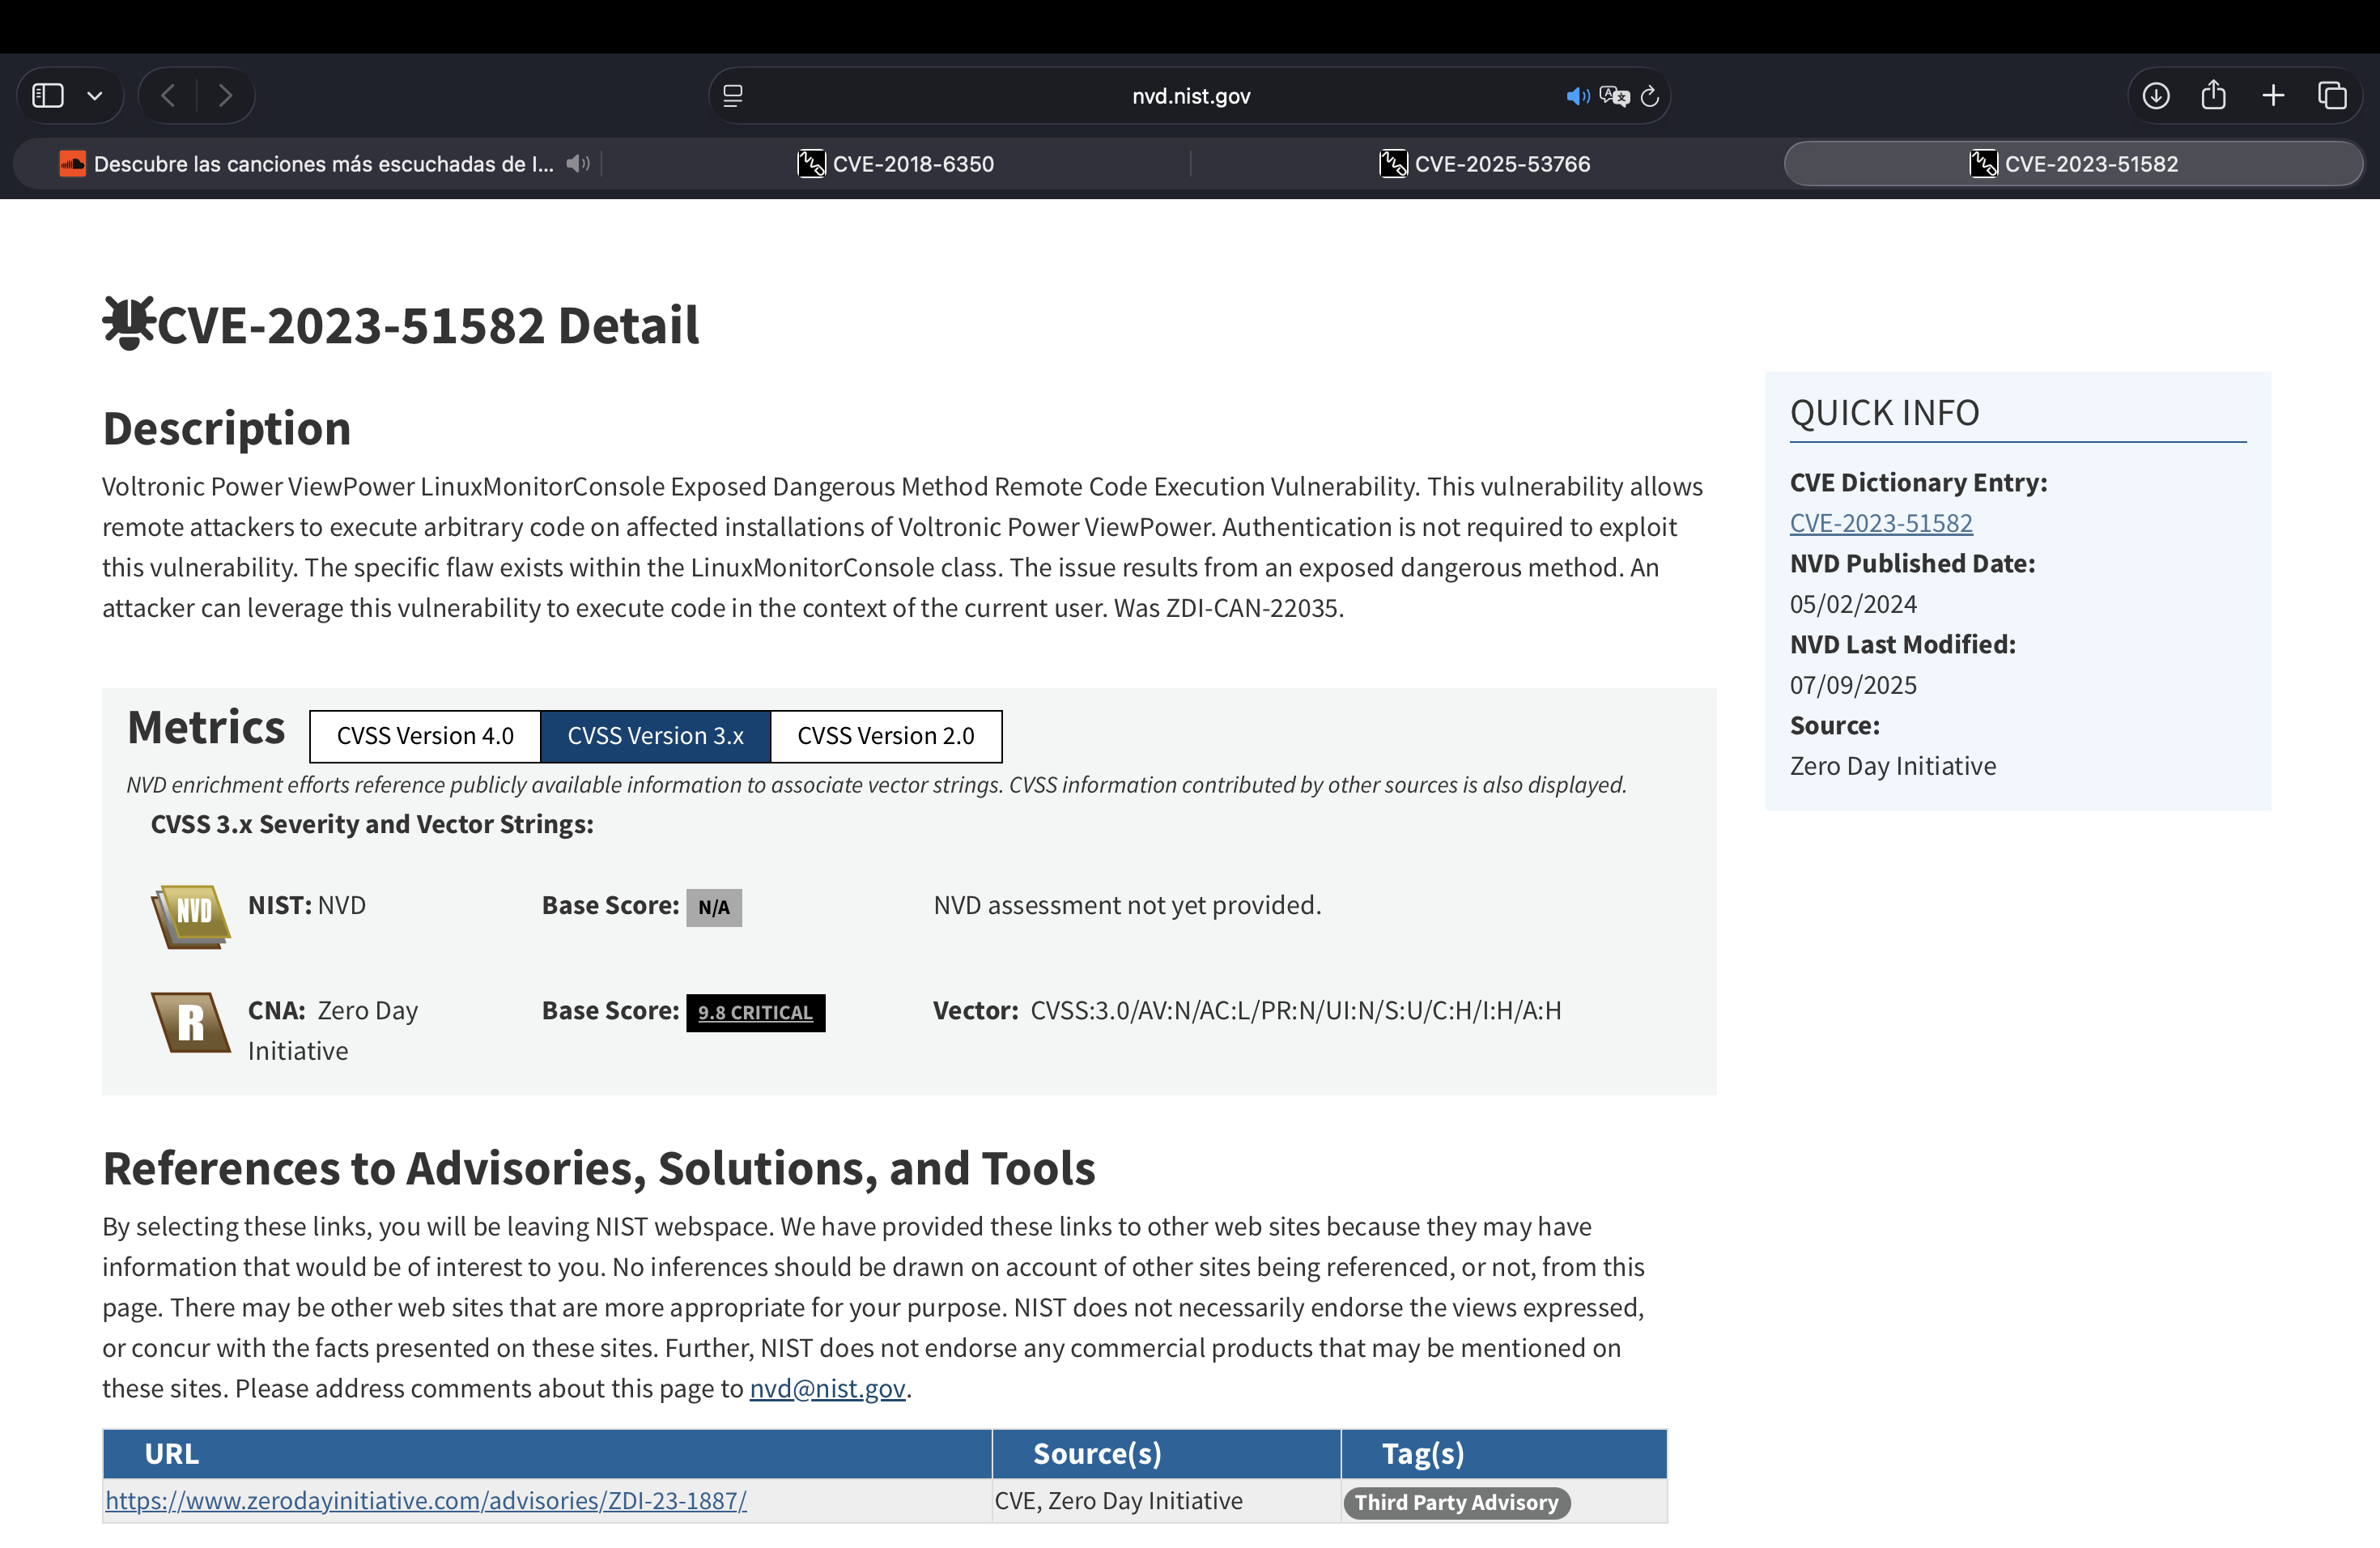
\includegraphics[width=0.95\textwidth]{Imagenes/07-CVE-3.png}
    \caption{Detalle de la CVE-2023-51582 en la NVD.}
    \label{fig:cve3}
\end{figure}
